\documentclass{article}
\usepackage[utf8]{inputenc}
\usepackage{amsmath}
\usepackage{enumitem}
\usepackage{graphicx} 
\author{Knoll Alexander}
\title{Numerik 2: Abgabe 1}
\usepackage{listings}
\lstloadlanguages{Python}
\date{24.04.2016}
\lstset{numbers=left,stepnumber=1,frame=single,language=Python,
        basicstyle=\scriptsize\ttfamily,numberstyle=\scriptsize,
        commentstyle=\upshape\ttfamily,
        numbersep=7pt,tabsize=2,breaklines=false,
        morecomment=[l]{//},showtabs=false,showspaces=false,
        showstringspaces=false,extendedchars=true,inputencoding={utf8},
        keywordstyle=\bfseries\color{darkblue},stringstyle=\color{darkred}}
\newcommand{\pp}[1]{\phantom{#1}}
\renewcommand{\theenumi}{\Alph{enumi}}
\newcommand\Section[1]{ %
  \addtocontents{toc}{\protect\setcounter{tocdepth}{0}}
  \subsubsection*{#1}
  \addtocontents{toc}{\protect\setcounter{tocdepth}{3}}}
\usepackage{color}
\definecolor{darkblue}{rgb}{0,0,.6}
\definecolor{darkred}{rgb}{.6,0,0}
\definecolor{darkgreen}{rgb}{0,.6,0}
\definecolor{red}{rgb}{.98,0,0}
\usepackage{caption,tabularx,booktabs}
\usepackage{multirow}
\usepackage{here} 
\renewcommand{\refname}{Literaturverzeichnis}
\renewcommand{\contentsname}{Inhaltsverzeichnis}




\begin{document}

\maketitle
\newpage
\tableofcontents
\newpage



\section{Aufgabe 1}

	\subsection{Mehrschrittverfahren untersuchen}
	
		Untersuchen Sie für die folgenden Mehrschrittverfahren, ob sie mindestens von der Ordnung 2
		sind (d. h. lokale Konsistenzordnung 3 besitzen) und ob sie stabil sind:
	
		\begin{enumerate}[label=(\alph*)]
			\item  $y_{i+1} = y_{i-1} + 2hf_{i}$ 
			\item  $y_{i+1}  = 3y_{i} - 2y_{i-1} + \frac{h}{12}[7f_{i+1} - 8f_{i} - 11f_{i-1}] $ 
			\item  $y_{i+1} = \frac{4}{3}y_{i} - \frac{1}{3}y_{i-1} + \frac{h}{9}[4f_{i+1} + 4f_{i} - 2f_{i-1}]$ 
		\end{enumerate}
		
		Zunächst sollen die Verfahren auf Stabilität hin untersucht. Hierfür werden characteristische Polynome aufgestellt und diese auf Nullstellen hin untersucht, wobei
		gilt $f(t, y) = 0$. Somit wird ersichtlich ob die Verfahren Nullstabil sind, oder nicht.
		
		\begin{align*}
			y_{i+1} - y_{i-1} = 0\\
			\mu^{2} - 0\mu - 1 \\
			\{ \mu_{1} = 1, \mu_{2} = -1\}
		\end{align*}
		
		Somit ist dieses Verfahren Nullstabil.
		
		\begin{align*}
			y_{i+1} - 3y_{i} + 2y_{i-1} = 0\\
			\mu^{2} - 3\mu + 2 \\
			\{ \mu_{1} = 1, \mu_{2} = 2\}
		\end{align*}
		
		Somit ist dieses Verfahren nicht Nullstabil.
		
		\begin{align*}
			y_{i+1} - \frac{4}{3}y_{i} + \frac{1}{3}y_{i-1} \\
			\mu^{2} - \frac{4}{3}\mu + \frac{1}{3} \\
			\{ \mu_{1} = \frac{1}{3}, \mu_{2} = 1\}
		\end{align*}
		
		Auch hier liegen die Lösungen im interval $[-1,1]$. Dies bedeutet dass auch dieses Verfahren Nullstabil ist.
		
		\Section{Taylor-Entwicklung}
		
		Durch Taylor-Entwicklung ist es möglich die Konsistenzordnung der jeweiligen verfahren zu bestimmen.
		\begin{align*}
			T(y(t_{i+1})) - T(y_{i+1}) = O(h^{p+1}) \\
			= \frac{1}{3}h^{3}y'''(t)
		\end{align*}
		
		Somit folgt dass dieses Verfahren nicht konsistent ist (konsistenz ordnung 0).
		
		\begin{align*}
			T(y(t_{i+1})) - T(y_{i+1}) = O(h^{p+1}) \\
			y + hy' + \frac{1}{2}h^{2}y'' + O(h^{3}) = 3y -2(y-hy' + \frac{1}{2}h^{2}+O(h^{2})) +\frac{h}{12}[7T(f_{i_+1}) -8y' -11T(f_{i-1})] \\
			= \frac{1}{6}h^{3}y''' + 3O(h^{3}) + \frac{1}{3}O(h^{4})
		\end{align*}
		
		Somit hat dieses Verfahren mindestens Konsistenzordnung 3.
		Abschließend wird dass letzte Verfahren untersucht
		
		\begin{align*}
			T(y(t_{i+1})) - T(y_{i+1}) = O(h^{p+1}) \\
			y + hy' + \frac{1}{2}h^{2}y'' + O(h^{3}) = \frac{4}{3}y -\frac{1}{3}(y-hy' + \frac{1}{2}h^{2}+O(h^{2})) +\frac{h}{9}[4T(f_{i_+1}) -4y' -2T(f_{i-1})] \\
			= \frac{h^{3}}{9}y''' - O(h^{3}) + \frac{2}{9}O(h^{4})
		\end{align*}
		
		Somit ist auch gezeigt, dass dieses Verfahren Konsistenzordnung 3 besitzt.
		

	
	\subsection{Verfahren implementieren}
	
		Implementieren Sie das erste der drei Verfahren sowie das Verfahren
		
		\begin{align*}
			y_{i+1} = \frac{4}{3}y_{i} - \frac{1}{3}y_{i-1} + \frac{2h}{3}f_{i+1}
		\end{align*}
		
		und verwenden Sie bei letzerem ein geeignetes Verfahren zum Lösen des nichtlinearen Gleichungssystems.
		
		\Section{Erstes Verfahren}
		
			Für das erste Verfahren ist es recht einfach einen algorithmus zu implementieren. Python selbst verwendet dynamische Datentypen und ermöglicht somit 
			die Übergabe von Funktionen (bzw. Methoden) als Parameter. Definiert wird eine routine $explicit_middle$, welche als argumente dass zu verwendende interval, die Schrittweite $h$,
			sowohl y' als funktion $f(t, y)$ und einen anfangswert $y(0)$ bekommt. Eine mögliche implementierung könnte wie folgt aussehen
			\newline
			

			\begin{tabular}{c}
			\begin{lstlisting}
			def explicit_middle(interval, f, h, y_0):

    		length = len(interval)
    		ys = [None for _ in range(length)]
    		ys[0] = y_0

				# anlaufrechnung mit dem expliziten euler verfahren
    		ys[1] = y_0 + h * f(interval[0], y_0)

    		for i in range(1, length-1, 1):
        		ys[i+1] = ys[i-1] + 2*h*f(interval[i], ys[i])

    		return ys
			\end{lstlisting}
 			\end{tabular}	
 			\newline
 			
 			Zurückgegeben werden die $y$-werte an den stützstellen des übergebenen intervals in form eines Arrays.
 			
 		\Section{Zweites Verfahren}
 		
 			Das zweite Verfahren lässt sich bereits nicht so einfach umsetzen wie das vorherige. Da auf beiden Seiten der Gleichung der Term $y_{i+1}$ vorkommt ist es notwendig ein weiteres lösungsverfahren, wie zum
 			Beispiel das Newton- oder dass Sekanten-Verfahren, einzubeziehen. Die routine nimmt die selben argumente wie das vorherige Verfahren auch. Als zusätliches lösungsverfahren wurde in der folgenden implementierung ein einfaches Sekanten-Verfahren gewählt.	
 			\newline
 			
 			\begin{tabular}{c}
 			\begin{lstlisting}
			def implicit_bdf(interval, f, h, y_0):

   				length = len(interval)
    			ys = [None for _ in range(length)]
    			ys[0] = y_0
					# anlaufrechnung mit dem expliziten euler verfahren
    			ys[1] = y_0 + h * f(interval[0], y_0)

    			for i in range(1, length-1, 1):
        			U = (ys[i-1], ys[i])
        			func2 = lambda u: u - 4/3 * ys[i] + 1/3 * ys[i-1] 
        										-  h * 2/3 * f(interval[i+1], u)
        										
        			# anwenden des sekanten verfahrens
       				ys[i+1] = U[1] - (U[1]-U[0])/(func2(U[1]) 
       											- func2(U[0]))*func2(U[1])
       				
		    	return ys
 			\end{lstlisting}
 			\end{tabular}	
 			\newline
 			
 			Durch iteratives anwenden des Sekantenverfahrens könnte die Genauigkeit weiter erhöt werden, erkauft wird diese Genauigkeit jedoch mit einem höheren Risiko für Auslöschung.
 			Wieder werden die $y$-werte in einem array zurückgegeben.
	
		
	\subsection{Numerische Lösung}
	
		Berechnen Sie (mit Python) numerische Lösungen mit $h = 1; 10^{-1} ; 10^{-2} , ...$ ausgehend von den exakten Startwerten für $y(0)$ und $y(h)$ für den Wert $y(10)$ und bestimmen Sie jeweils die Fehler. Bestimmen Sie daraus auch die Fehlerordnung und vergleichen Sie sie mit Ihrem theoretischen Ergebnis.
		
		Um die verfahren tatsächlich auszuwerten wird eine Testgleichung benötigt.
		Mithilfe dieser bestimmen wir den exakten Wert für $y(10)$ und vergleichen diesen mit den numerischen. Dabei werden die Schrittweiten
		$h = 1; 10^{-1} ; 10^{-2}; 10^{-3}, 10^{-4}$ und $10^{-5}$ verwendet. Die betrachtete Differentialgleichung ist hierbei $\dot{y} = -2y(t) + 1$, mit dem anfangsbedingung $y(0) = 1$.
		Die Auswertung des Verfahresfehlers an der Stelle $t = 10$ liefert folgende Tabelle (das Erste Verfahren wird mit A bezeichnet, dass Zweite mit B). Mithilfe von wolfram alpha
		wird der exakte Wert der Lösung auf $y(10) = 0.5000000010305768$ festgelegt
		\newline
		
		\begin{table}[!h]
		\centering
		\begin{tabular}{c c c c}
			\bf h & \bf A & \bf B \\
			\hline
			$1$ & -257114.49 & 9.70059897618114e-05\\
			$10^{-1}$ & -2066217.22 & 3.1363700525588456e-10 \\
			$10^{-2}$ & -24218.67 & 3.101852108500225e-12 \\
			$10^{-3}$ & -242.57 & 4.929390229335695e-14 \\
			$10^{-4}$ & -2.42 & 2.0106138975961585e-13 \\
			$10^{-5}$ & -0.024257224873262873 & 2.679634292235278e-12 \\
		\end{tabular}
		\end{table}
		
		Aus obiger Tabelle wird ersichtlich wie ungeeignet Verfahren A zur Lösung des gestellten Problems ist. Es besteht immer die möglichkeit dass sich fehler in der Umsetzung des numerischen Verfahrens einschleichen, wenn es jedoch um die Wahl der Methode geht, so ist liegt man in diesem Fall mit Verfahren B auf der sicheren Seite. Durch die Theoretischen überlegungen war bereits klar dass das erste Verfahren
		nicht gegen die Lösung konvergieren wird, da es nicht konsistent ist.
		
	\subsection{Anfangswertproblem untersuchen}
	
		Gegeben ist das Anfangswertproblem
	
		\begin{align}
			\dot{y} = -2y(t) + 1 , y(0) = 1
		\end{align}
		
		Bestimmen sie die exakte Lösung des AWPs und vergleichen Sie sie mit der numerischen.

		\subsubsection{Analytische Lösung}
		
			Zunächste muss Gleichung (1) in Standart Notation gebracht werden, welche gegeben ist durch:
			
			\begin{align*}
				\dot{y} + p(t) = Q(t)
			\end{align*}
			
			Somit kann Gleichung (1) überführt werden in
			
			\begin{align}
				\dot{y} + 2y = 1
			\end{align}
			
			Eine allgemeine lösung zu einer Gleichung in Standart Notation kann mithilfe folgender ausdrücke bestimmt werden
			
			\begin{align*}
				u(x) = e^{\int p(x) dt} \\
				\frac{d}{dt}(uy) = Q(t)
			\end{align*}
			
			Angewandt auf Gleichung (2) erhält man einen Ausdruck welcher durch beidseitiges integrieren und weiterem umformen, die
			allgemeine Lösung des Problems beschreibt.
			
			\begin{align*}
				u = e^{\int 2 dt}\\
				\frac{d}{dt}(e^{2t}y) = e^{2t} && | \int \\
				\int \frac{d}{dt}(e^{2t}y) = \int e^{2t} \\
				e^{2t}y = \frac{1}{2}e^{2t} + C && | \div e^{2t} \\
				y = \frac{1}{2} + \frac{C}{e^{2t}} \\
				y = \frac{1}{2} + Ce^{-2t}
			\end{align*}
			
			Einbeziehen der Anfangsbedingung $y(0) = 1$ liefert die exakte Lösung des Problems
			
			\begin{align*}
				y(0) = \frac{1}{2} + C*e^{-2*0} \\
				1 = \frac{1}{2} + C && | - \frac{1}{2} \\
				\frac{1}{2} = C
			\end{align*}
			\newpage
			Und somit die exakte Lösung
			
			\begin{align}
				y(t) = \frac{1}{2}e^{-2t} + \frac{1}{2}
			\end{align}
			
			\begin{figure}[H] 
			  \centering
			     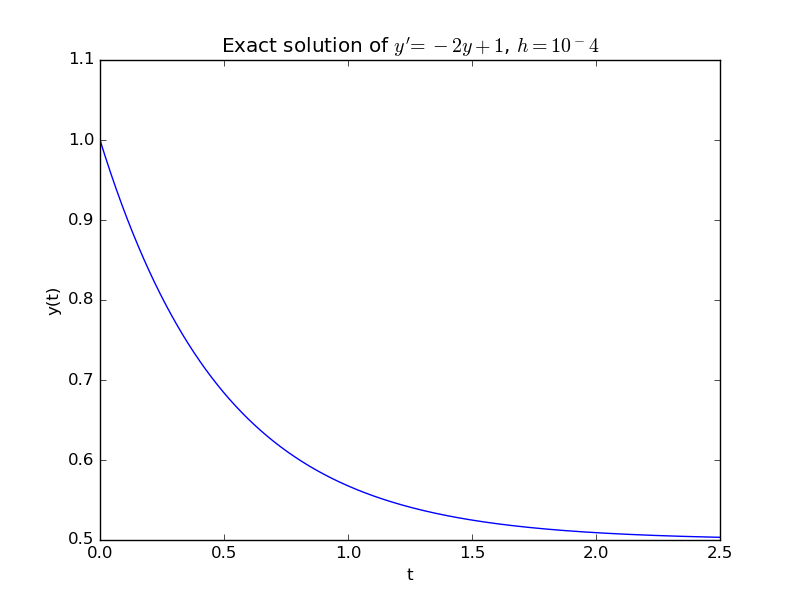
\includegraphics[width=0.7\textwidth]{analytic_solution.png}
			  \caption{Analytische lösung im Intervall [0; 2,5]}
			  \label{fig:Bild1}
			\end{figure}
			
			Wenn nun Störungungen in die Anfangsbedingung eingeführt werden, kann man das Problem auf stabilität untersuchen. Hierfür wird
			,ausgehend von der allgemeinen lösung, eine exakte Lösung unter verwendung von $y(0) = 1 + \epsilon$ bestimmt.
			
			\begin{align*}
				y_{\epsilon}(t) = (\frac{1}{2} + \epsilon)e^{-2t} + \frac{1}{2}
			\end{align*}
			
			Es ist leicht zu sehen dass für sehr kleine $\epsilon$, die lösung keine größeren abweichungen erfährt.
			Somit kann die Lösung als Stabil bezeichnet werden. 
			
		\subsubsection{Numerische Lösung}
		
			Als folge der stabilität des AWPs, ist es sehr wahrscheinlich dass Einschrittverfahren für ausreichend kleine $h$ gegen die Lösung des Problems konvergieren. Deshalb soll im folgend der vergleich dreier Verfahren, die Schrittweite $h=0,5$ genutzt werden. Dies liefert eine bessere visuelle darstellung der tatsächlichen unterschiede der genutzen Verfahren. Genutzt werden dass implizite und explizite Euler-Verfahren als auch dass Adams-Moultan-Verfahren (Ordnung 2).
			
			\Section{Expliziter Euler}
			
				Das Verfahren wird beschrieben durch
				
				\begin{align*}
					u_{i+1} = u_{i} + hf_{i}
				\end{align*}
				
				angewandt auf Gleichung (1) erhält man
				
				\begin{align*}
					y_{i+1} = y_{i} + h(-2y_{i}+1) \\
					y_{i+1} = (1-2h)y_{i} + h
				\end{align*}
			
			\Section{Impliziter Euler}
			
				Das implizite verfahren lautet wie folgt.
				
				\begin{align*}
					u_{i+1} = u_{i} + hf_{i+1}
				\end{align*}
				
				Da $y' = f(t, y)$ bekannt ist es möglich dass verfahren durch umformungen auf eine einfach
				auswertbare Form zu bringen. Andernfalls wäre es notwendig in jedem iterations-schritt ein passendes
				Lösungsverfahren anzuwenden, wie beispielsweise dass Newton-Verfahren oder dass Sekanten-Verfahren.
				
				\begin{align*}
					y_{i+1} = y_{i} + h(-2y_{i+1}+1) \\
					y_{i+1} = y_{i} - 2hy_{i+1} + h  && | +2hy_{i+1} \\
					(1+2h)y_{i+1} = y_{i} + h && | \div(1+2h) \\
					y_{i+1} =  \frac{y_{i} + h}{1+2h}
				\end{align*} 
			
			\Section{Adams-Moultan}
			
				Dieses Verfahren existieren in verschiedenen Variationen. In diesem Fall wird die Methode der 2. Ordnung verwendet.
				
				\begin{align*}
					u_{i+1} = u_{i} + \frac{h}{2}[f_{i+1} + f_{i}]
				\end{align*}
				
				Wie bereits beim implizieten Euler Verfahren, ist es möglich die gleichung in eine einfach auswertbare form zu
				bringen.
				
				\begin{align*}
					y_{i+1} = y_{i} + \frac{h}{2}[-2y_{i+1} + 1 - 2y_{i+1} + 1] \\
					y_{i+1} = y_{i} - hy_{i+1} - hy_{i} + h && | +hy_{i+1} \\
					(1+h)y_{i+1} = (1-h)y_{i} + h && | \div(1+h) \\
					y_{i+1} = \frac{(1-h)y_{i}+h}{1+h}
				\end{align*}
				
			
			\Section{Vergleich}
			
				Unter einbezug von Python werden die resultate visualisiert.
				
				\begin{figure}[htbp] 
					\centering
					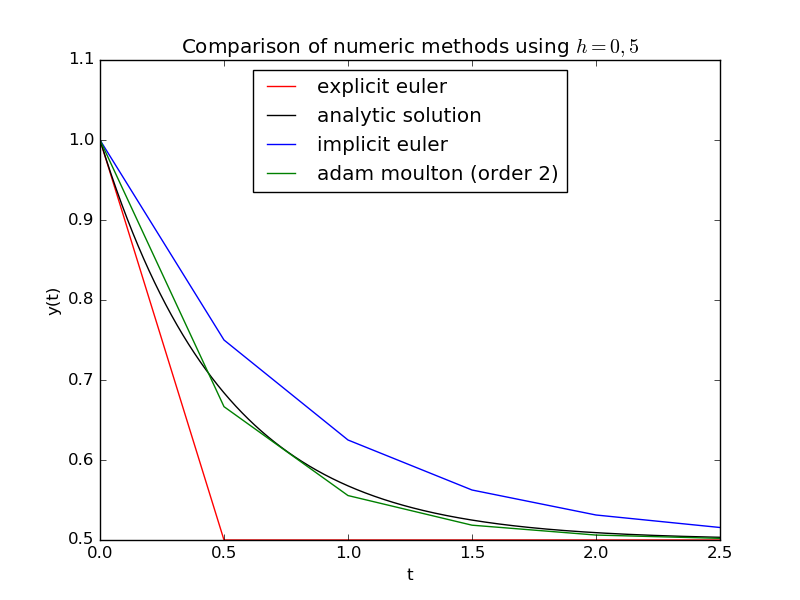
\includegraphics[width=0.7\textwidth]{numeric_plots.png}
					\caption{Vergleich der Numerischen Lösungen mit der Analytischen}
					\label{fig:Bild2}
				\end{figure}
			
				Die Grafik zeigt deutlich, dass jedes der angewandten Verfahren letztendlich gegen die Lösung konvergiert.
				Jedoch konvergieren die Einschritt-Verfahren wesentlich langsamer als das Adams-Moultan-Verfahren, welches 
				selbst für recht große $h$ einen guten eindruck macht. Weiterhin scheint es so als würde dass expliziete Euler-Verfahre direkt nach dem ersten iterations schritt auf 0 fallen, wodurch es unbrauchbar wird. Abhilfe schafft eine kleinere Wahl von $h$.
				
				\newpage
				
				\begin{figure}[htbp] 
					\centering
					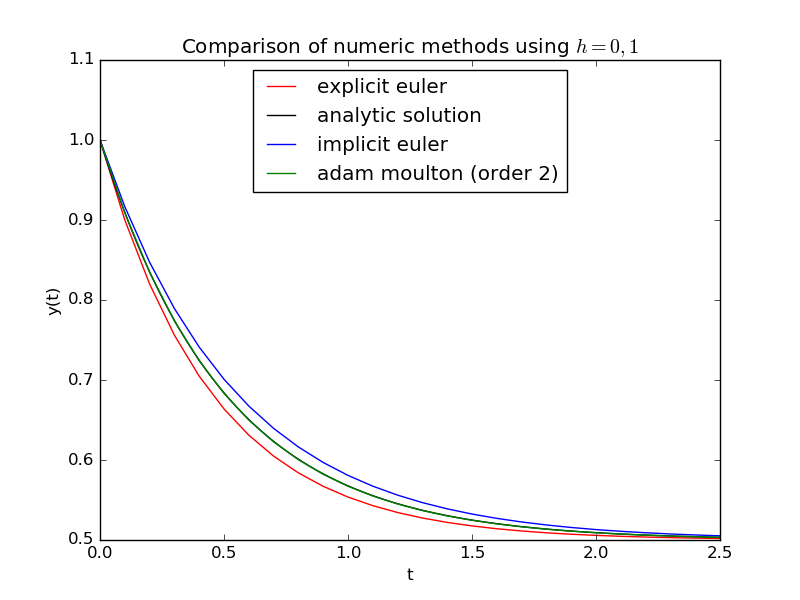
\includegraphics[width=0.7\textwidth]{numeric_plots2.png}
					\caption{Numerische Lösungen mit kleinerem h}
					\label{fig:Bild3}
				\end{figure}
				
				In der obigen Abbildung wird deutlich, wie gut das Adams-Moultan-Verfahren für das AWP geeignet ist.
				
				
				
\newpage				
	\subsection{Stellungnahme}
	
		$Knoll Alexamder: $ Mein Teil an der Umsetzung war die Bearbeitung der kompletten Zweiten Aufgabe, als auch der dokumentation in TeX. Teil der Umsetzung war die Implementierung der Python files "two.py" und "four.py".		
				

\begin{thebibliography}{xxxxxxxxxxxxxxxxxxxxxxxxxxxxxxxxxxxxxx}
   \bibitem[http://www2.mathematik.hu-berlin.de/~gaggle/W0506/MATHINF/HANDOUT/handout4-4n.pdf]{}
   \bibitem[http://math-www.uni-paderborn.de/~walter/teachingSS04/VortragThema5.pdf]{}
\end{thebibliography}
	
\end{document}

